\chapter{Auswertung}
\label{cha:Auswertung}

Nun möchte ich die Auswertung der Daten anhand von einer mehrwöchigen Aufzeichnung im Klassenzimmer demonstrieren.

\section{Aufzeichnung}
\label{auswertung_aufzeichnung}

Zu Beginn des Schuljahrs 2014/15 habe ich meine Messtation am 8.9.2014 in der Klasse aufgebaut. Die Messung ging mit nur einigen Minuten Unterbrechung bis zum 3.10.2014. Hierbei wurden ungefähr 2 Mal in der Minute 10 Sensoren ausgelesen. Die dabei entstandene \gls{CSV}, hat 75875 Zeilen und ist knapp über \SI{6}{\mega\byte} groß.\footnote{Sie kann unter \href{http://winkler.kremszeile.at/dygraph_8A.csv}{winkler.kremszeile.at/dygraph\_8A.csv} heruntergeladen werden.}

\section{Graphische Darstellung}

Die Messdaten lassen sich sehr einfach auswerten, wenn man sie als Diagramme darstellt (siehe \ref{subsec:Diagramme}).\footnote{Für die interaktive Ansicht: \href{http://winkler.kremszeile.at/dygraphs_au\%C3\%9Fen.html\#dygraph8A.csv}{winkler.kremszeile.at/dygraphs\_außen.html\#dygraph8A.csv}}

So merkt man bei den meisten Sensoren, dass die Werte alle 24 Stunden periodisch schwanken. Am besten ist das bei der Luftfeuchtigkeit zu erkennen, welche zwischen ca. \SI{60}{\%} (Mittag bis Abend) und \SI{100}{\%.rel.LF} (Mitternacht bis Vormittag) schwankt. (siehe Abbildungen \ref{fig:auswertung-aussen} und \ref{fig:auswertung-temperaturen}).
Da das Klassenzimmer außerhalb des Unterrichts nicht geheizt wird und die Wände des Containers kaum isolieren, schwankt auch die Innentemperatur an Schultagen sehr stark. Verstärkt wird dies dadurch, dass der Temperatursensor auf der Seite des Raumes befestigt war, an dem auch die Fenster und Heizkörper sind. Es ist auch erkennbar, dass es an Wochenenden deutlich kälter  ist, da nicht geheizt wird. 
Erstaunlich ist jedoch, dass die Temperaturschwankungen sogar an der \gls{CPU}-Temperatur deutlich erkennbar sind. (siehe Abbildung \ref{fig:auswertung-cpu})

Am ungenauesten sind die Ergebnisse des Luftqualitätssensors. Diese enthalten viele Ausreißer und sind im Allgemeinen viel zu hoch. Die Originalsoftware gibt in den Standardeinstellungen bei einem Wert von 1500 die Warnung \enquote{Bad air quality} an. Im Klassenzimmer wurden jedoch häufig Werte über 2000 gemessen. (siehe Abbildung \ref{fig:auswertung-qualitat}) Erkennbar ist jedoch, dass die Luftqualität erwartungsgemäß im Laufe des Vormittags immer  schlechter wird und sich nachmittags langsam wieder erholt. 

\begin{figure}[p]
  \centering
     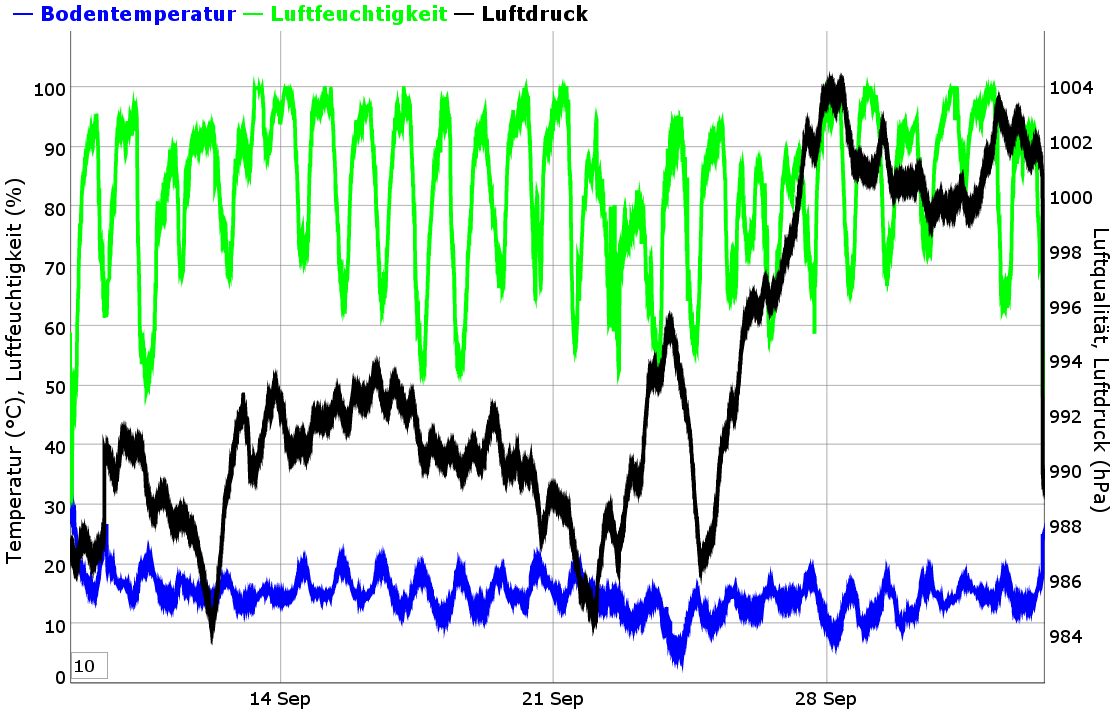
\includegraphics[width=0.95\textheight, angle=90]{figures/auswertung-aussen.png}
  \caption{Außensensoren}
  \label{fig:auswertung-aussen}
\end{figure}

\begin{figure}[p]
  \centering
     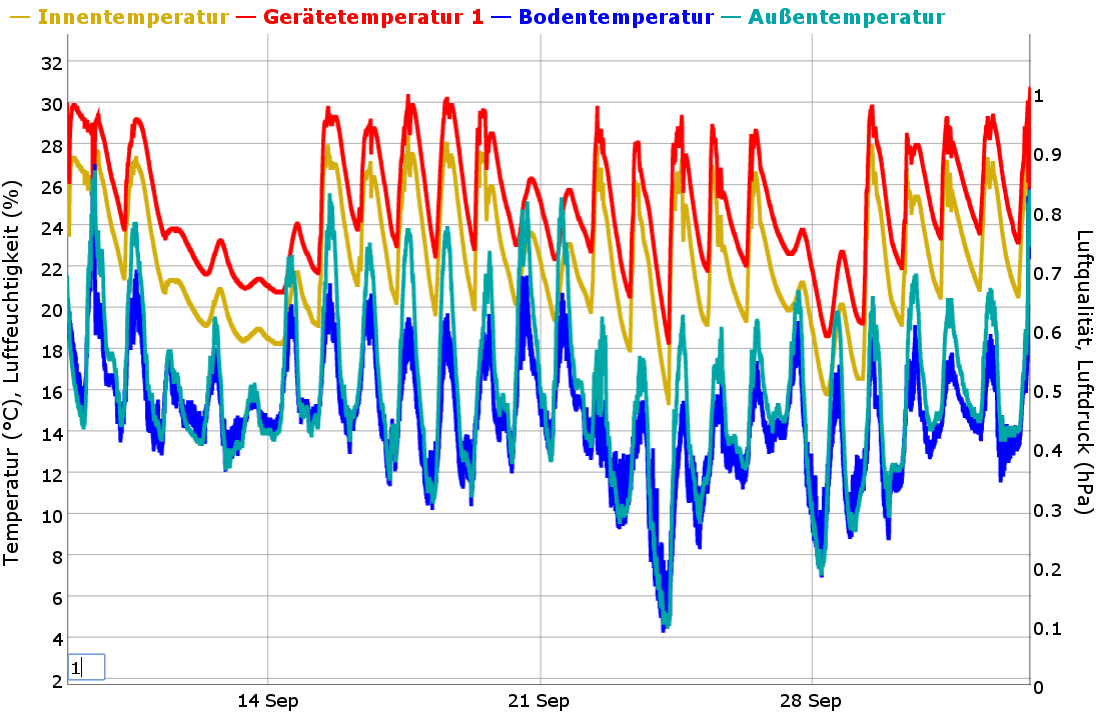
\includegraphics[width=0.95\textheight, angle=90]{figures/auswertung-temperaturen.png}
  \caption{Temperatursensoren}
  \label{fig:auswertung-temperaturen}
\end{figure}

\begin{figure}[h]
  \centering
     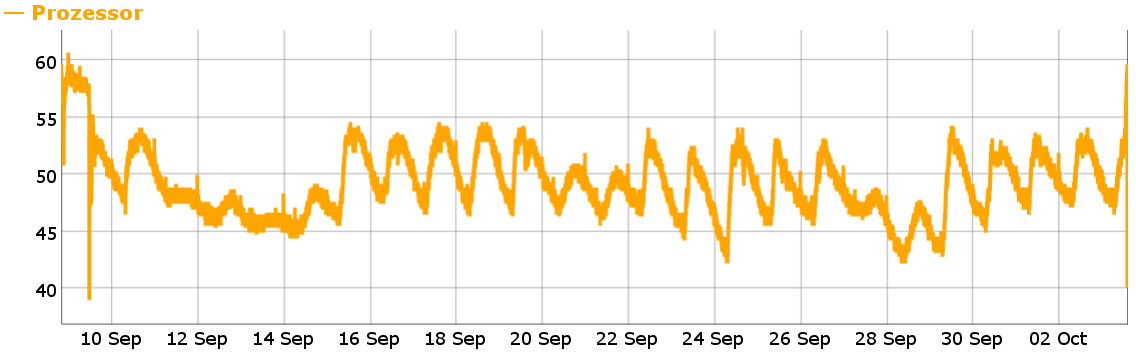
\includegraphics[width=\textwidth]{figures/auswertung-cpu.png}
  \caption{\gls{CPU}-Temperatur}
  \label{fig:auswertung-cpu}
\end{figure}

\begin{figure}[h]
  \centering
     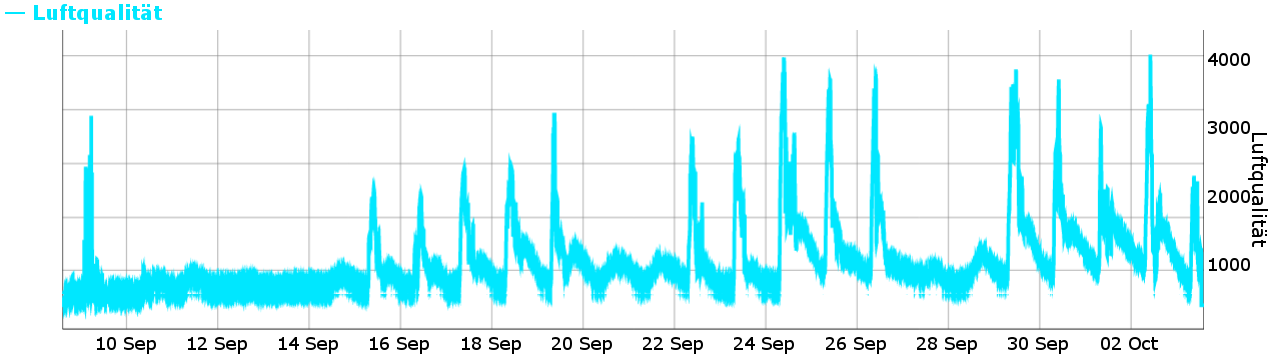
\includegraphics[width=\textwidth]{figures/auswertung-qualitat.png}
  \caption{Luftqualität}
  \label{fig:auswertung-qualitat}
\end{figure}

\newpage

\section{Endauswertung}
\label{auswertung_endauswerung}

\begin{tabulary}{\textwidth}{c|c|C|C|C|C}
Sensor & Einheit & Mittelwert & Minimum & Maximum & \gls{Standardabweichung} \\
\hline
Innentemperatur & \si{\degreeCelsius} & 22.43 & 15.375 & 30.875 & 2.94 \\ 
\hline
Gerätetemperatur 1 & \si{\degreeCelsius} & 25.00 & 18.312 & 34.312 & 2.82 \\ 
\hline
Gerätetemperatur 2 & \si{\degreeCelsius} & 25.01 & 18.25 & 34.375 & 2.82 \\ 
\hline
Bodentemperatur & \si{\degreeCelsius} & 14.69 & 4.312 & 29.312 & 2.90 \\ 
\hline
Außentemperatur & \si{\degreeCelsius} & 15.94 & 4.5 & 39.0 & 3.96 \\ 
\hline
Außentemperatur 2 & \si{\degreeCelsius} & 15.84 & 3.5 & 33.2 & 3.86 \\ 
\hline
Luftfeuchtigkeit & \% rel. LF & 83.03 & 14.7 & 99.9 & 12.54 \\ 
\hline
Luftdruck & \si{\hecto\glslink{Pascal}{\pascal}} & 993.27 & 984.04 & 1004.12 & 5.27 \\ 
\hline
Prozessor & \si{\degreeCelsius} & 49.33 & 39.0 & 62.1 & 3.04 \\ 
\hline
Qualität & rel. Wert & 1027.29 & 450.0 & 5870.0 & 529.88 \\ 
\end{tabulary}
